\documentclass[]{article}
\usepackage{lmodern}
\usepackage{amssymb,amsmath}
\usepackage{ifxetex,ifluatex}
\usepackage{fixltx2e} % provides \textsubscript
\ifnum 0\ifxetex 1\fi\ifluatex 1\fi=0 % if pdftex
  \usepackage[T1]{fontenc}
  \usepackage[utf8]{inputenc}
\else % if luatex or xelatex
  \ifxetex
    \usepackage{mathspec}
  \else
    \usepackage{fontspec}
  \fi
  \defaultfontfeatures{Ligatures=TeX,Scale=MatchLowercase}
\fi
% use upquote if available, for straight quotes in verbatim environments
\IfFileExists{upquote.sty}{\usepackage{upquote}}{}
% use microtype if available
\IfFileExists{microtype.sty}{%
\usepackage{microtype}
\UseMicrotypeSet[protrusion]{basicmath} % disable protrusion for tt fonts
}{}
\usepackage[margin=1in]{geometry}
\usepackage{hyperref}
\hypersetup{unicode=true,
            pdftitle={写在美国民主党2020大选党内辩论之前},
            pdfauthor={李泉},
            pdfborder={0 0 0},
            breaklinks=true}
\urlstyle{same}  % don't use monospace font for urls
\usepackage{graphicx,grffile}
\makeatletter
\def\maxwidth{\ifdim\Gin@nat@width>\linewidth\linewidth\else\Gin@nat@width\fi}
\def\maxheight{\ifdim\Gin@nat@height>\textheight\textheight\else\Gin@nat@height\fi}
\makeatother
% Scale images if necessary, so that they will not overflow the page
% margins by default, and it is still possible to overwrite the defaults
% using explicit options in \includegraphics[width, height, ...]{}
\setkeys{Gin}{width=\maxwidth,height=\maxheight,keepaspectratio}
\IfFileExists{parskip.sty}{%
\usepackage{parskip}
}{% else
\setlength{\parindent}{0pt}
\setlength{\parskip}{6pt plus 2pt minus 1pt}
}
\setlength{\emergencystretch}{3em}  % prevent overfull lines
\providecommand{\tightlist}{%
  \setlength{\itemsep}{0pt}\setlength{\parskip}{0pt}}
\setcounter{secnumdepth}{0}
% Redefines (sub)paragraphs to behave more like sections
\ifx\paragraph\undefined\else
\let\oldparagraph\paragraph
\renewcommand{\paragraph}[1]{\oldparagraph{#1}\mbox{}}
\fi
\ifx\subparagraph\undefined\else
\let\oldsubparagraph\subparagraph
\renewcommand{\subparagraph}[1]{\oldsubparagraph{#1}\mbox{}}
\fi

%%% Use protect on footnotes to avoid problems with footnotes in titles
\let\rmarkdownfootnote\footnote%
\def\footnote{\protect\rmarkdownfootnote}

%%% Change title format to be more compact
\usepackage{titling}

% Create subtitle command for use in maketitle
\providecommand{\subtitle}[1]{
  \posttitle{
    \begin{center}\large#1\end{center}
    }
}

\setlength{\droptitle}{-2em}

  \title{写在美国民主党2020大选党内辩论之前}
    \pretitle{\vspace{\droptitle}\centering\huge}
  \posttitle{\par}
    \author{李泉}
    \preauthor{\centering\large\emph}
  \postauthor{\par}
      \predate{\centering\large\emph}
  \postdate{\par}
    \date{2019-06-26}

\usepackage{booktabs}
\usepackage{longtable}
\usepackage{array}
\usepackage{multirow}
\usepackage{wrapfig}
\usepackage{float}
\usepackage{colortbl}
\usepackage{pdflscape}
\usepackage{tabu}
\usepackage{threeparttable}
\usepackage{threeparttablex}
\usepackage[normalem]{ulem}
\usepackage{makecell}
\usepackage{xcolor}

\begin{document}
\maketitle

特朗普6月18号在奥兰多集会正式宣布拉开连任竞选大幕。这边厢民主党的第一次党内参选人辩论也将于6月26号在迈阿密开始。由于符合参加辩论门槛的参选人有20位,所以将分两天进行,一次10人。

民主党方面目前所有宣布参加初选的一共有24位参选人,他们的基本信息按照英文字母顺序列在下表:

\begin{table}[H]
\centering
\begin{tabular}{l|l|l|l|l|l}
\hline
候选人 & 姓名 & 年龄 & 参选时间 & 经历 & 主张\\
\hline
![Michael Bennet](/Users/BillyJack/Documents/HomeFiles/US Elections Project/bennet-2.png)\{width=40\%\} & Michael Bennet/贝内特 & 54 & 2019.5.2 & 科罗拉多州参议员 & 加大基建投资,2013年曾参与起草移民改革法\\
\hline
![Joseph R. Biden](/Users/BillyJack/Documents/HomeFiles/US Elections Project/biden.png)\{width=40\%\} & Joseph R. Biden Jr./拜登 & 76 & 2019.4.25 & 特拉华州参议员,副总统 & 重建美国的世界地位,恢复制造业\\
\hline
![Cory Booker](/Users/BillyJack/Documents/HomeFiles/US Elections Project/booker-2.png)\{width=40\%\} & Cory Booker/布克 & 50 & 2019.2.1 & 新泽西州联邦参议员 & 刑事司法改革,团结国家,奥巴马范\\
\hline
![Steve Bullock](/Users/BillyJack/Documents/HomeFiles/US Elections Project/bullock-2.png)\{width=40\%\} & Steve Bullock/布洛克 & 53 & 2019.5.14 & 蒙大拿州州长 & 竞选献金改革,加强幼儿早教\\
\hline
![Pete Buttigieg](/Users/BillyJack/Documents/HomeFiles/US Elections Project/buttigieg-2.png)\{width=40\%\} & Pete Buttigieg/布蒂吉格 & 37 & 2019.4.14 & 印第安纳州南岸市市长,老兵 & 应对气候变化,经济机会,主打新世代牌\\
\hline
![Julian Castro](/Users/BillyJack/Documents/HomeFiles/US Elections Project/castro-2.png)\{width=40\%\} & Julian Castro/卡斯特罗 & 44 & 2019.1.12 & 圣安东尼奥市前市长,前联邦住房部部长 & 普惠学前教育,普惠医疗,移民改革\\
\hline
![bill de Blasio](/Users/BillyJack/Documents/HomeFiles/US Elections Project/blasio-2.png)\{width=40\%\} & Bill de Blasio/布拉西奥 & 58 & 2019.5.16 & 纽约市市长 & 加强学前教育\\
\hline
![John Delaney](/Users/BillyJack/Documents/HomeFiles/US Elections Project/delaney-2.png)\{width=40\%\} & John Delaney/德莱尼 & 56 & 2017.7.28 & 马里兰州前众议员 & 普惠医保\\
\hline
![Tulsi Gabbard](/Users/BillyJack/Documents/HomeFiles/US Elections Project/gabbard-2.png)\{width=40\%\} & Tulsi Gabbard/加伯德 & 38 & 2019.1.17 & 夏威夷州联邦众议员,国民警卫队老兵 & 反对海外军事干涉\\
\hline
![Kirsten Gillibrand](/Users/BillyJack/Documents/HomeFiles/US Elections Project/gillibrand-2.png)\{width=40\%\} & Kirsten Gillibrand/吉列布兰德 & 52 & 2019. 1.15 & 纽约州联邦参议员 & 女性平权\\
\hline
![Kamala Harris](/Users/BillyJack/Documents/HomeFiles/US Elections Project/harris-2.png)\{width=40\%\} & Kamala Harris/哈里斯 & 54 & 2019.1.21 & 加州联邦参议员、加州前司法部长 & 为中产阶级减税、民权议题\\
\hline
![John Hickenlooper](/Users/BillyJack/Documents/HomeFiles/US Elections Project/hickenlooper-2.png)\{width=40\%\} & John Hickenlooper/希肯卢珀 & 67 & 2919.3.4 & 科罗拉多州前州长 & 扩大低收入人群医保,同性恋权利和枪支管制\\
\hline
![Jay Inslee](/Users/BillyJack/Documents/HomeFiles/US Elections Project/inslee-2.png)\{width=40\%\} & Jay Inslee/英斯利 & 68 & 2019.3.1 & 华盛顿州州长 & 应对气候变化,可再生能源\\
\hline
![Amy Klobuchar](/Users/BillyJack/Documents/HomeFiles/US Elections Project/klobuchar-2.png)\{width=40\%\} & Amy Klobuchar/克洛巴查 & 59 & 2019.2.10 & 明尼苏达州联邦参议员 & 应对阿片和毒品滥用危机,降低药价\\
\hline
![Wayne Messam](/Users/BillyJack/Documents/HomeFiles/US Elections Project/messam.png)\{width=40\%\} & Wayne Messam/梅瑟姆 & 45 & 2019.3.28 & 佛罗里达州Miramar市市长 & 取消4400万美国人1.5万亿的学生贷款\\
\hline
![Seth Moulton](/Users/BillyJack/Documents/HomeFiles/US Elections Project/moulton-2.png)\{width=40\%\} & Seth Moulton/莫尔顿 & 40 & 219.4.22 & 麻省联邦众议员,伊战老兵 & 新对外政策和国家安全及防务政策\\
\hline
![Beto O'Rourke](/Users/BillyJack/Documents/HomeFiles/US Elections Project/orourke-2.png)\{width=40\%\} & Beto O'Rourke/奥罗克 & 46 & 2019.3.14 & 前得州联邦众议员 & 移民改革,大麻合法化,农村医疗\\
\hline
![Tim Ryan](/Users/BillyJack/Documents/HomeFiles/US Elections Project/ryan-2.png)\{width=40\%\} & Tim Ryan/瑞安 & 45 & 2019.4.4 & 俄亥俄州联邦众议员 & 修订贸易协议,打击中国操纵货币,加强工会权利\\
\hline
![Bernie Sanders](/Users/BillyJack/Documents/HomeFiles/US Elections Project/sanders-2.png)\{width=40\%\} & Bernie Sanders/桑德斯 & 77 & 2019.2.19 & 佛蒙特州联邦参议员 & 民主社会主义者,全民医保,大学免费,绿色新政,15美元最低时薪\\
\hline
![Joe Sestak](/Users/BillyJack/Documents/HomeFiles/US Elections Project/sestak.png)\{width=40\%\} & Joe Sestak/塞斯塔克 & 67 & 2019.6.23 & 宾州前联邦众议员,退役海军上将 & 应对气候变化,重振美国的世界地位\\
\hline
![Eric Swalwell](/Users/BillyJack/Documents/HomeFiles/US Elections Project/swalwell-2.png)\{width=40\%\} & Eric Swalwell/斯沃韦尔 & 38 & 2019.4.8 & 加州联邦众议员 & 全国禁止攻击性武器,加大医学研究\\
\hline
![Elizabeth Warren](/Users/BillyJack/Documents/HomeFiles/US Elections Project/warren-2.png)\{width=40\%\} & Elizabeth Warren/沃伦 & 70 & 2019.2.9 & 麻省联邦参议员,哈佛大学教授 & 反对大公司和政治腐败导致的收入不平等\\
\hline
![Marianne Williamson](/Users/BillyJack/Documents/HomeFiles/US Elections Project/williamson-2.png)\{width=40\%\} & Marianne Williamson/威廉森 & 66 & 2019.1.30 & 畅销书作家 & 为奴隶制赔偿1000亿美元\\
\hline
![Andrew Yang](/Users/BillyJack/Documents/HomeFiles/US Elections Project/yang-2.png)\{width=40\%\} & Andrew Yang/杨 & 44 & 2017.11.6 & 前高科技公司老板 & 每人每月1000美元基本收入\\
\hline
\end{tabular}
\end{table}

根据民主党全国委员会设定的门槛,参选人如果能够在三个被民主党认定的民调中获得至少1\%的支持,或者得到65000不同人的捐款,并且这些捐款来自至少20个州中至少200人,就可以参加第一次辩论。按照这个标准,上述24人当中20人符合条件。

和特朗普的集会在能坐2万人的体育馆不同,这次的辩论会场在一个只能容纳2200人的表演中心。谁能作为观众参加全部由民主党全国委员会决定,基本就局限在所有佛州和迈阿密当地的民主党政要、重要的捐款人和掌握票仓的民间组织领导人这三个群体中间。

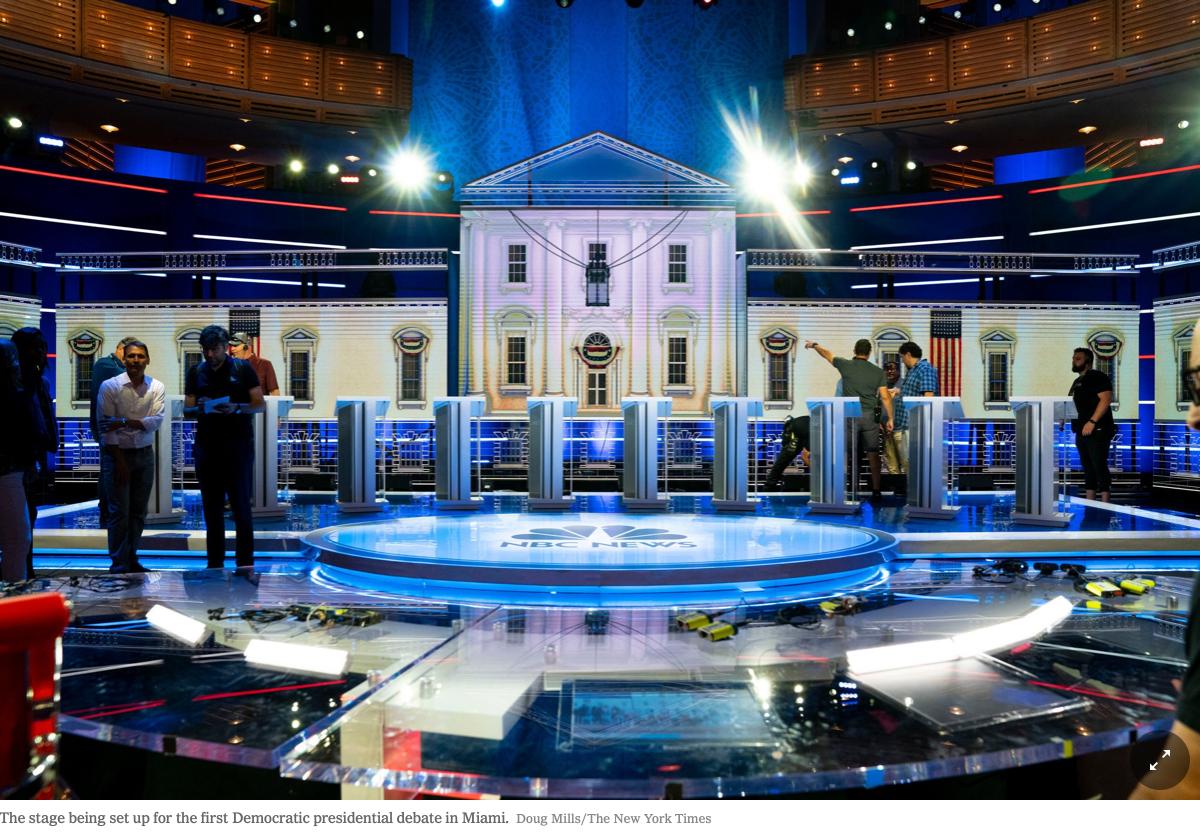
\includegraphics{/Users/BillyJack/Documents/HomeFiles/US Elections Project/debatescene.png}

符合门槛要求的20人根据抽签决定参加26或者27号的辩论。那么26号参加的10人在舞台上从左到右分别是:

\begin{tabular}{l|l|l|l|l|l|l|l|l|l}
\hline
布拉西奥 & 瑞安 & 卡斯特罗 & 布克 & 沃伦 & 奥罗克 & 克洛巴查 & 加伯德 & 英斯利 & 德莱尼\\
\hline
![](/Users/BillyJack/Documents/HomeFiles/US Elections Project/blasio-2.png)\{width=40\%\} & ![](/Users/BillyJack/Documents/HomeFiles/US Elections Project/ryan-2.png)\{width=40\%\} & ![](/Users/BillyJack/Documents/HomeFiles/US Elections Project/castro-2.png)\{width=40\%\} & ![](/Users/BillyJack/Documents/HomeFiles/US Elections Project/booker-2.png)\{width=40\%\} & ![](/Users/BillyJack/Documents/HomeFiles/US Elections Project/warren-2.png)\{width=40\%\} & ![](/Users/BillyJack/Documents/HomeFiles/US Elections Project/orourke-2.png)\{width=40\%\} & ![](/Users/BillyJack/Documents/HomeFiles/US Elections Project/klobuchar-2.png)\{width=40\%\} & ![](/Users/BillyJack/Documents/HomeFiles/US Elections Project/gabbard-2.png)\{width=40\%\} & ![](/Users/BillyJack/Documents/HomeFiles/US Elections Project/inslee-2.png)\{width=40\%\} & ![](/Users/BillyJack/Documents/HomeFiles/US Elections Project/delaney-2.png)\{width=40\%\}\\
\hline
\end{tabular}

27号参加的10个人的占位从左至右是:

\begin{tabular}{l|l|l|l|l|l|l|l|l|l}
\hline
威廉森 & 希肯卢珀 & 杨 & 布蒂吉格 & 拜登 & 桑德斯 & 哈里斯 & 吉列布兰德 & 贝内特 & 斯沃韦尔\\
\hline
![](/Users/BillyJack/Documents/HomeFiles/US Elections Project/williamson-2.png)\{width=40\%\} & ![](/Users/BillyJack/Documents/HomeFiles/US Elections Project/hickenlooper-2.png)\{width=40\%\} & ![](/Users/BillyJack/Documents/HomeFiles/US Elections Project/yang-2.png)\{width=40\%\} & ![](/Users/BillyJack/Documents/HomeFiles/US Elections Project/buttigieg-2.png)\{width=40\%\} & ![](/Users/BillyJack/Documents/HomeFiles/US Elections Project/biden.png)\{width=40\%\} & ![](/Users/BillyJack/Documents/HomeFiles/US Elections Project/sanders-2.png)\{width=40\%\} & ![](/Users/BillyJack/Documents/HomeFiles/US Elections Project/harris-2.png)\{width=40\%\} & ![](/Users/BillyJack/Documents/HomeFiles/US Elections Project/gillibrand-2.png)\{width=40\%\} & ![](/Users/BillyJack/Documents/HomeFiles/US Elections Project/bennet-2.png)\{width=40\%\} & ![](/Users/BillyJack/Documents/HomeFiles/US Elections Project/swalwell-2.png)\{width=40\%\}\\
\hline
\end{tabular}

从两天的重量级人物分布来看,27号要重于26号。第一天辩论中的重量级人物只有麻省联邦参议员沃伦。而拜登、桑德斯等都集中在第二天。

根据CNN6月21号民调支持度的排名,目前参选24人中排在前十位的分别是拜登,沃伦,桑德斯,哈里斯,布蒂吉格,奥罗克,布克,克落巴查,杨和卡斯特罗。

从这些参选人在美国政治光谱上的占位分布而言,Businessinsider做了一个调查,让受访者对民主党的这些参选者按照其所了解到的进步主义倾向的浓厚程度打分。根据调查结果再运用最大似然算法给所有人做了一个排序。从图中可以看出,桑德斯作为自许的社会主义者,在受访者心目中立场最为激进,沃伦的进步主义色彩强于拜登,而进步主义色彩最弱的则是四次到过伊拉克战场的莫尔顿。

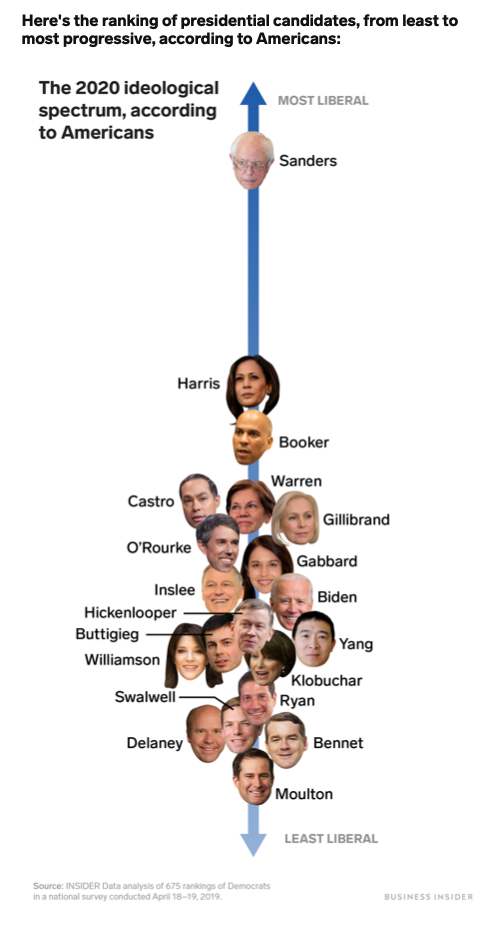
\includegraphics{/Users/BillyJack/Documents/HomeFiles/US Elections Project/ranking2.png}

第一张表中列出的主要是这些参选人的国内政策立场。从对外政策的角度来看,Vox网站考虑了四个代表性人物:拜登和布蒂吉格属于传统阵营,希望维持美国在国际事务方面的传统超强地位。桑德斯和沃伦属于进步主义阵营,想改革现有的国际经济秩序,因为他们认为现有的安排造成了全球的收入的巨大不平等。不过他们两人并不反对美国在全球保持领导地位。

民主党现在面临的最大问题是还没有找出能整合其支持者的参选人。要想重新上台,民主党在选人方面有两个策略可以考虑。一是挑选一位能积聚人气,以打败特朗普为中心而忽略政策立场的候选人。这个策略的危险之处在于会最大程度地继续撕裂美国选民。二是找一位政策立场适中,能够通过政策来催动选民支持的候选人。这个策略的危险之处在于具体政策的效用在当今以候选人为中心的选举模式下非常有限,面对特朗普这样的媒体鼓动达人,希拉里2016年选择第二个策略从结果而言是失败的。那么有没有两方面都结合的好的候选人呢?很可惜,现在看来没有。21世纪最缺什么?人才!


\end{document}
